% !TeX spellcheck = en_US
\documentclass[11pt,xcolor=dvipsnames,professionalfonts]{beamer}

% Pakete
\usepackage[utf8]{inputenc}
\usepackage[english]{babel}

% AMS Pakete
\usepackage{amsmath}
\usepackage{amsfonts}
\usepackage{amssymb}
\usepackage{mathtools}

% Text tools
\usepackage{textcomp}

% Einheiten
\usepackage{siunitx}
\sisetup{
	separate-uncertainty
}

% Grafiken
\usepackage{graphicx}
\usepackage{booktabs}
\usepackage{multirow}
\setbeamerfont{caption}{size=\footnotesize}
\setbeamertemplate{caption}{\raggedright\insertcaption\par}
\usepackage[percent]{overpic}

% Theme
\usetheme{Boadilla}
\usecolortheme{rose}
\useoutertheme{infolines}
\useinnertheme{rectangles}
\setbeamertemplate{itemize subitem}[triangle]

\usefonttheme[onlymath]{serif}

% [num] Zitationen
\setbeamertemplate{bibliography item}[text]

% Navigationsleiste ausschalten
\beamertemplatenavigationsymbolsempty

\author[Christian Bespin \& Christopher Deutsch]
{Christian Bespin \& Christopher Deutsch}

\title
{Analysis of $\mathrm{Z}^0$ Decays}

\subtitle
{}
%\logo{}

\institute[]
{Advanced Laboratory Course\\ Summer Term 16}

\date{May 30, 2016}

%\setbeamercovered{transparent}
%\setbeamertemplate{navigation symbols}{}

\newcommand{\beginbackup}{
	\newcounter{framenumbervorappendix}
	\setcounter{framenumbervorappendix}{\value{framenumber}}
}
\newcommand{\backupend}{
	\addtocounter{framenumbervorappendix}{-\value{framenumber}}
	\addtocounter{framenumber}{\value{framenumbervorappendix}} 
}

\begin{document}
\maketitle


\begin{frame}{Outline}
	\tableofcontents
\end{frame}

\section{Introduction}
\begin{frame}{Christian's Folien}
	Hier deine Folien
\end{frame}

\section{Theoretical Background}

\section{Part I: Analysis of Event Displays}

\section{Part II: Statistical Analysis of $\mathrm{Z}^0$ Decays}
\begin{frame}{Part II: Statistical Analysis of $\mathrm{Z}^0$ Decays}
	\begin{itemize}
		\setlength\itemsep{2.em}
		\item Analysis of data gathered by OPAL at LEP
		\begin{itemize}
			\setlength\itemsep{0.5em}
			\item event displays infeasible ($\sim \num{400000}$ events)
			\item data analysis software \texttt{PAW} used instead
		\end{itemize}
		
		\item Determination of
		\begin{itemize}
			\setlength\itemsep{0.5em}
			\item cross sections $\sigma_f$
			
			\item electroweak mixing $\sin^2\theta_\mathrm{W}$ (forward-backward asymmetry)
			
			\item mass $M_\mathrm{Z}$ and total decay-width $\Gamma_\mathrm{Z}$
			
			\item partial decay-widths $\Gamma_f$ (lepton universality, number of light neutrino generations $N_\nu$)
		\end{itemize}
	\end{itemize}
\end{frame}

\begin{frame}{Part II: Statistical Analysis of $\mathrm{Z}^0$ Decays}
	\textbf{Procedure:}
	\begin{enumerate}
		\setlength\itemsep{2.em}
		\item Analysis of Monte-Carlo data
		\begin{itemize}
			\setlength\itemsep{0.5em}
			\item refine selection cuts for the different decay-channels
			
			\item separate $s$- and $t$-channel in $\mathrm{e}^+ + \mathrm{e}^- \rightarrow \mathrm{e}^+ + \mathrm{e}^-$
			
			\item determine the efficiency of the applied cuts
		\end{itemize}
		
		\item Analysis of OPAL data
		\begin{itemize}
			\setlength\itemsep{0.5em}
			\item separate the decay-channels with the selection cuts
			
			\item efficiency formalism to obtain the total number of events
			
			\item calculation of the physical quantities
		\end{itemize}
	\end{enumerate}
\end{frame}

\subsection{Analysis of Monte-Carlo Data}

\begin{frame}{Analysis of Monte-Carlo Data}
	\begin{itemize}
		\setlength\itemsep{2.em}
		\item Simulated events with detector response separated into decay channels $\mathrm{e}, \mu, \tau, \mathrm{q}$ (\num{100000} events each)
		
		\item Available variables for each event:
		\begin{description}
			\item[\texttt{ncharged}] number of charged particles
			\item[\texttt{pcharged}] total momentum of charged particles
			\item[\texttt{e\_ecal}] total energy deposited in em.\ calorimeter
			\item[\texttt{e\_hcal}] total energy deposited in had.\ calorimeter
			\item[\texttt{cos\_thet}] angle between inc.\ and outg.\ positively charged particle
		\end{description}
	\end{itemize}
\end{frame}

\begin{frame}{Acceptance of the OPAL-Detector}
	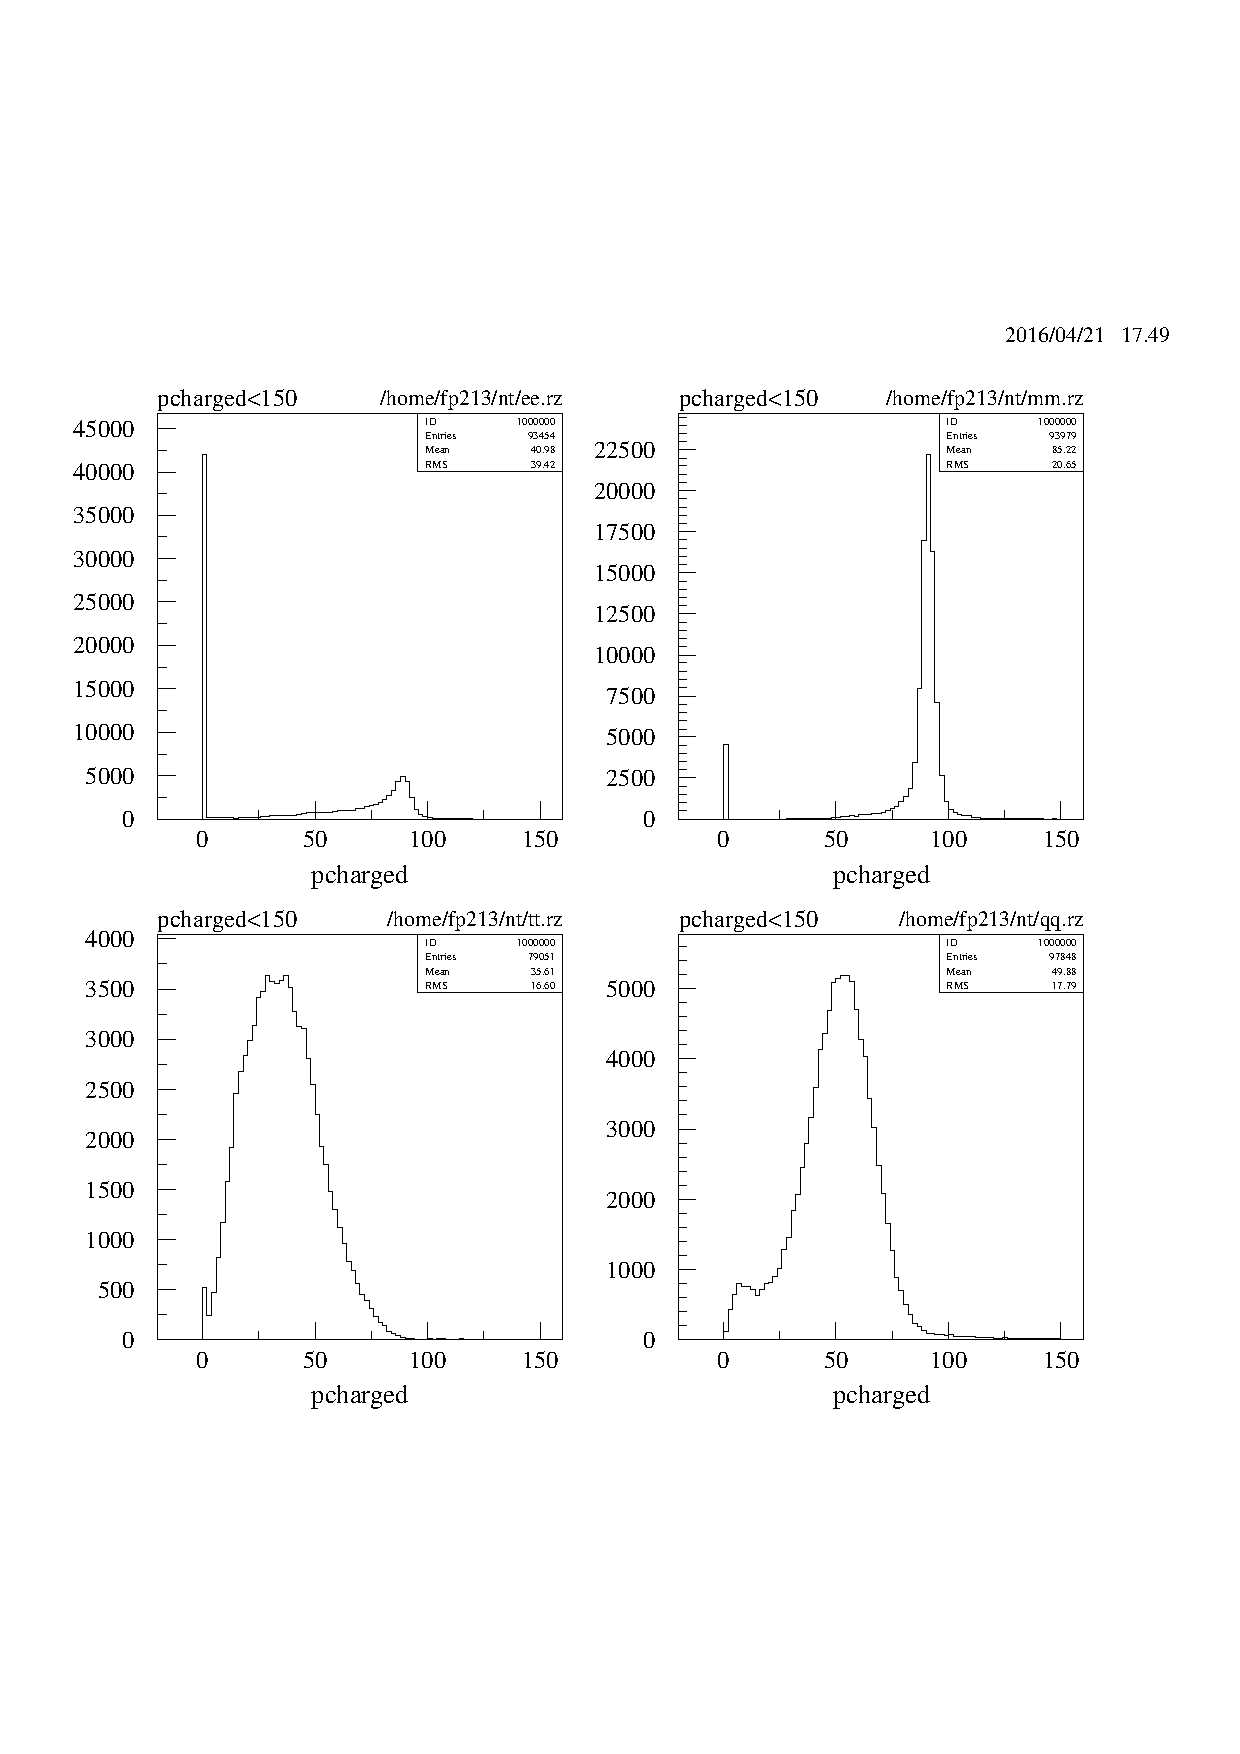
\includegraphics[height=0.9\textheight, trim=0 0 0 20, clip]{./data/tag2/uncut/cropped/pcharged_uncut.pdf}
\end{frame}

\begin{frame}
	\begin{itemize}
		\item Total number of events in each channel known
		\begin{itemize}
			\setlength\itemsep{0.5em}
			\item determination of efficiency
			\item probability of misidentification
		\end{itemize}
	\end{itemize}
\end{frame}

\subsection{Analysis of OPAL Data}

\section{Conclusion}

\begin{frame}
	\begin{center}
		\LARGE
		\textbf{Thank you for your attention!}
	\end{center}
\end{frame}

\begin{frame}{Bibliography}
	\scriptsize
	\begin{thebibliography}{9}
		\bibitem[PDG]{pdg}
			K.A. Olive \textit{et al.} (Particle Data Group),
			\emph{The Review of Particle Physics},
			Chin.\ Phys.\ C, \textbf{38}, 090001 (2014) and 2015 update.
	\end{thebibliography}
\end{frame}

\beginbackup

\begin{frame}{Backup Slides}
	Backup Slides
\end{frame}

\backupend

\end{document}